\paragraph{}
After the geometry information is exported from the IGES file, it can be feed into the quad-tree algorithm to generate mesh of the problem domain.
As an algorithm based on computational geometry, it require great amount of numerical operation and hence the result may be sensitive to the tolerance.
An absolute tolerance may not be able to handle problem with very large or small geometric size.
As a consequence, the first step is to normalize the geometry into a uniform space ($10\times10$ is used in this chapter).

\subsection{Background mesh}
\label{qdt_sc:qdt_background_mesh}
\paragraph{}
Background mesh describes a mesh in the background. %fig
Its density is decided by the geometry.
This section will introduce the procedure to generate the background mesh.
\paragraph{}
First of all, we start with one square which is the root of the tree.
The size of it will be slightly larger than the normalized input geometry and it is selected as $16 \times 16$ in this chapter.
After that, the root square will be divided into millions (defined by resolution, defined as $2^{res} \times 2^{res}$) smaller ones like pixels in the image.
Then, $2^{s_{max}} \times 2^{s_{max}}$ ``pixels'' will be group into the first layer of the tree, or initial background mesh as shown in fig.~\ref{qdt_fig:qdt_initial_mesh}.
It is used to control the maximum allowable mesh size globally or separately for different material regions.

\begin{figure}[!ht]
    \centering
    \scalebox{0.8}{
        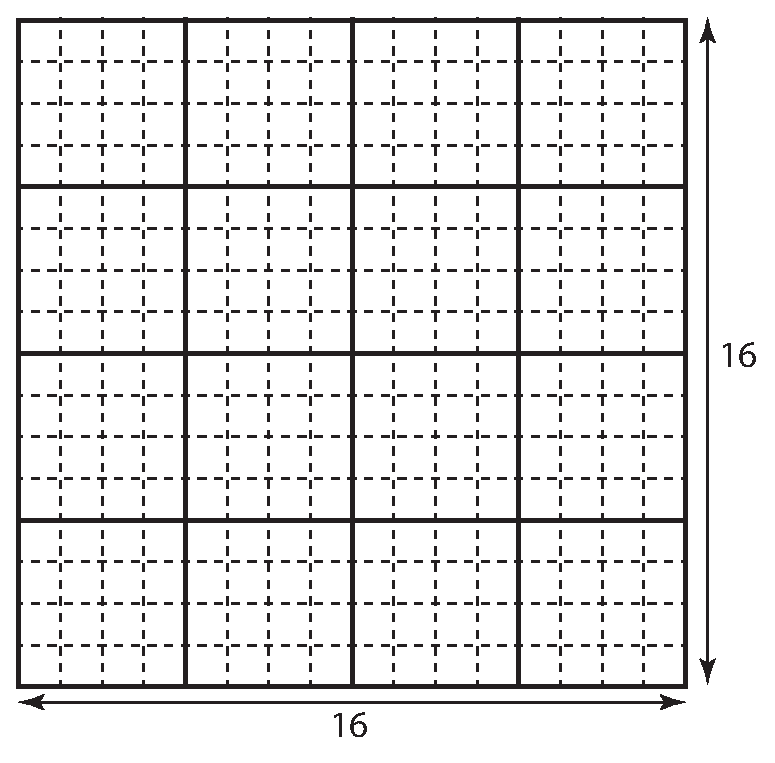
\includegraphics{quadtree/images/qdt_initial_mesh.eps}
    }
    \caption{An example of the background initial mesh: $16 \times 16$ square are divided into $2^4 \times 2^4$ pixels (dashed lines, $res=4$) and $2^2 \times 2^2$ pixels form the initial mesh (solid lines, $s_{max}=2$)}
    \label{qdt_fig:qdt_initial_mesh}
\end{figure}

\paragraph{}
% generating the initial mesh without balance
Criteria to decided whether each individual square in the initial mesh need to be refined or not is the seed points.
The curve will be uniformly discretized into a given number of seed points uniformly and the mesh will be refined until the number of the seed points within the square is less than the threshold.
However, finer mesh is expected at the region where geometry with high curvature appeared but the uniform discretization does not generate different number of points based on curvature.
It can be solved by treating each segment of the polylines as an individual curve when generating seed points.
Due to the fact that algorithm described in .~\ref{qdt_section:iges_output} guarantee the chord length to arc length ratio, polylines ought to have finer segments at the position where curvature is significant.

\paragraph{}
% only two intersections allowed
Although seed points provides a good guide on the mesh density, situations where high density mesh is required while few seed points appeared may happen as plotted in fig.~\ref{qdt_fig:qdt_seed_point_problem}.
The geometry limits the seed points due to the lack of curvature.
While, it is expected that the square element will be refined at least once as one layer of mesh may not be appropriate to formulate a thin shell structure. 
    \begin{figure}[!ht]
        \centering
        \scalebox{1}{
            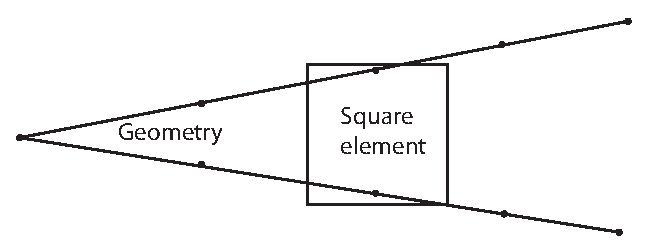
\includegraphics{quadtree/images/qdt_seed_points_problem}
        }
        \caption[Limitation of the seed points]{
            Limitation of the seed points: few seed points will be generated over a straight line and few seed points will be included in the square element which leads to unexpected behavior.
            \tikz\draw[black,fill=black] (0,0) circle (.7ex);
            stands for the seed points.
        }
        \label{qdt_fig:qdt_seed_point_problem}
    \end{figure}
As a result, another restriction will be adopted together with the seed points to prevent this kind of situation from happening.
Element with more than two unique intersections will be tagged to be refined no matter how many seed points it contains.
In numerical calculation, two points may be regarded as one if they are close enough to each others.
Normalization of the geometry described at the beginning of this section helps to define a meaningful tolerance to handle numerical error.



% balance the initial mesh
\paragraph{}
% balance in tree data structure
Self-balancing is adopted by most of the tree data structure such as AVL, B/B+, Red-black tree and so on.
Fig.~\ref{qdt_fig:tree_balance_avl} illustrates a self-balancing of an AVL tree.
Balancing by rotation is performed because difference in height of the leaf B and L is greater than the threshold.
    \begin{figure}
        \centering
        \scalebox{0.25}{
            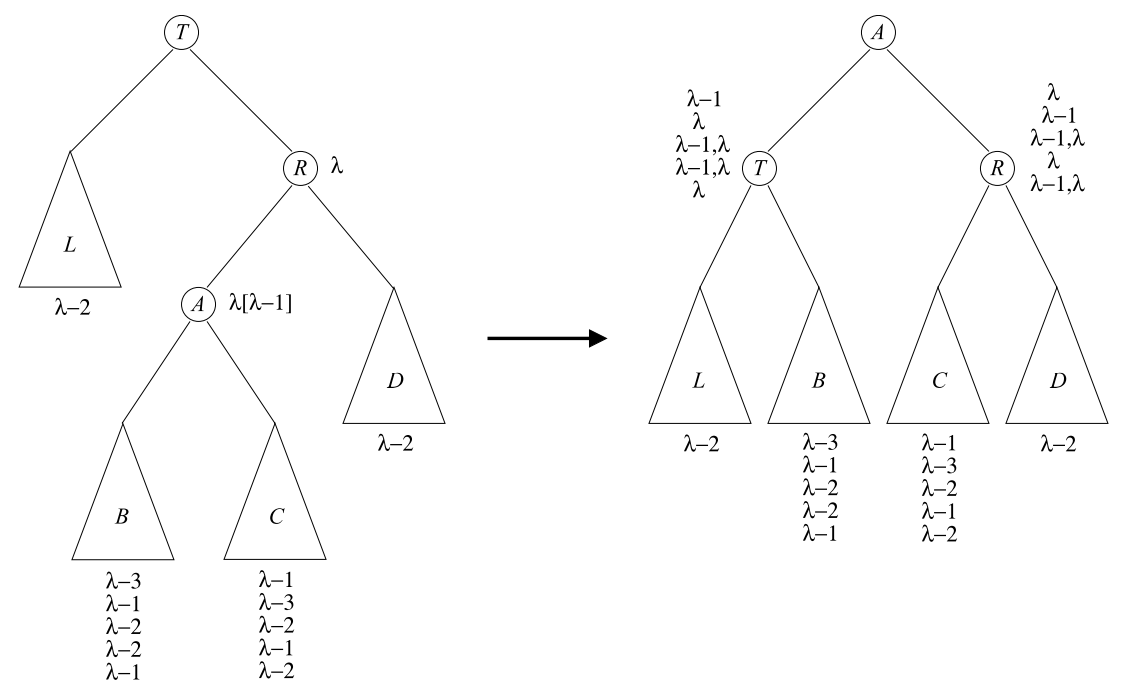
\includegraphics{quadtree/images/qdt_avl_balance.png}
        }
        \caption{Balance of the AVL tree \cite{Roura2013}}
        \label{qdt_fig:tree_balance_avl}
    \end{figure}

\paragraph{}
% balance in quadtree
Same idea is adopted in quadtree as well.
a refinement will be performed to achieve a balanced tree if the difference in the height of the leaf (Cell A and B in fig.~\ref{qdt_fig:tree_balance_quadtree} for example) is larger than one.
    \begin{figure}[!ht]
        \begin{subfigure}[b]{0.5\linewidth}
            \centering
            \scalebox{0.8}{
                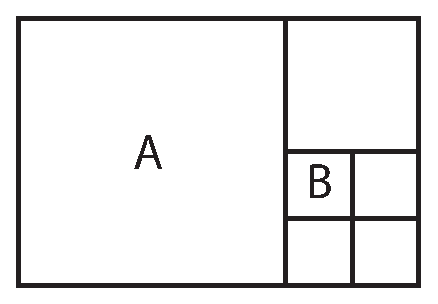
\includegraphics{quadtree/images/qdt_balance_before.eps}
            }
            \caption{Before balance operation}
        \end{subfigure}
        \begin{subfigure}[b]{0.5\linewidth}
            \centering
            \scalebox{0.8}{
                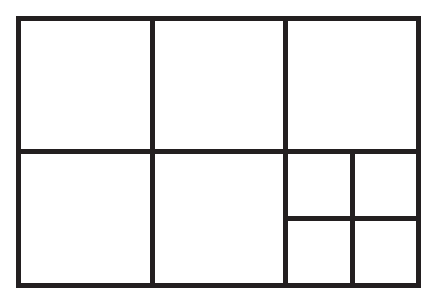
\includegraphics{quadtree/images/qdt_balance_after.eps}
            }
            \caption{After balance operation}
        \end{subfigure}
        \caption{Balance of quadtree: cell A is refined in order to balance the quadtree.}
        \label{qdt_fig:tree_balance_quadtree}
    \end{figure}

\paragraph{}
% reason behind balancing
The reason why balancing is predominately adopted in tree data structure lies in the guarantee of an $O\left(log(n)\right)$ time complexity for searching in any case.
Even thought computational cost on searching seems not to be significant during mesh generation using quadtree, a balanced tree provided some other attractive features that can be utilized in numerical analysis.
One of the advantages is to improve the mesh quality.
Any extremely small or large angle between the element and the scaling center may result in a bad quality mesh.
Chances are that these poor quality mesh may appear without self-balancing, fig.~\ref{qdt_fig:sbfem_adv_1} for an example.
    \begin{figure}[!ht]
        \centering
        \scalebox{1}{
            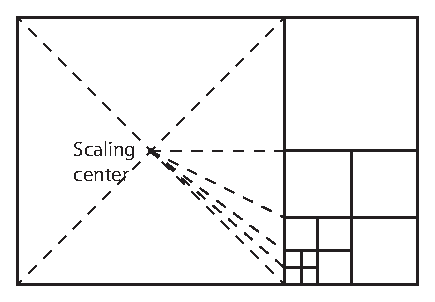
\includegraphics{quadtree/images/qdt_balance_sbfem_adv_1.eps}
        }
        \caption{Small angle between element and scaling center may reduce the mesh quality}
        \label{qdt_fig:sbfem_adv_1}
    \end{figure}

Another reason is to kept the pattern of the cells.
If the threshold of the self-balancing is set to one ($2:1$ ratio), only six kinds of cells will appear before the cutting as illustrated in fig.~\ref{qdt_fig:sbfem_adv_2}.
Thanks to the geometric similarity, local stiffness matrix can be calculated and scaled directly when same kind of the cell appears which significantly reduce the computational cost.
Hanging nodes in fig.~\ref{qdt_fig:sbfem_adv_2} can be a problem for traditional finite element to handle the displacement compatibility \cite{Tabarraei:2009:XFE} \cite{NME:NME3070} \cite{NME:NME2900} .
Solution including triangulation \cite{4037344} \cite{BERN1994384} \cite{ijeas251083} , using special shape function \cite{NME:NME1620120104} and other methods are available but special treatment is required.
As a comparison, SBFEM provides greater flexibility on the element, n-sides polygons with hanging nodes or curved edge can be treated natively.
    \begin{figure}[!ht]
        \centering
        \scalebox{1}{
            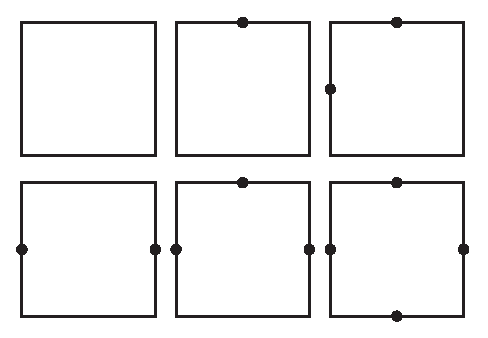
\includegraphics{quadtree/images/qdt_balance_sbfem_adv_2.eps}
        }
        \caption[Types of the cell in self-balancing quadtree]{
            Types of the cell when $2:1$ ratio is applied,
            \tikz\draw[black,fill=black] (0,0) circle (.7ex);
            stands for the hanging node
            }
        \label{qdt_fig:sbfem_adv_2}
    \end{figure}


\pagebreak


%=====================================================================================================================%
\subsection{Hard point treatment}
\paragraph{}
%introduction
Hard point is a kind of point in the geometry that must be meshed as a node or scaling center.
When more than two materials are involved, it is common to have some hard points to make sure the point shared by three material can be properly formulated as shown in fig.~\ref{qdt_fig:qdt_hard_point_demo}
    \begin{figure}[!ht]
        \begin{subfigure}[b]{0.5\linewidth}
            \centering
            \scalebox{0.8}{
                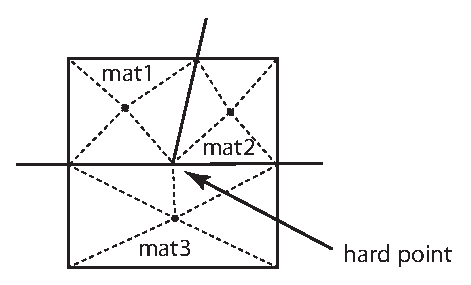
\includegraphics{quadtree/images/qdt_hard_point_demo.eps}
            }
        \caption{Hard point is meshed as node}
        \end{subfigure}
        \begin{subfigure}[b]{0.5\linewidth}
            \centering
            \scalebox{0.8}{
                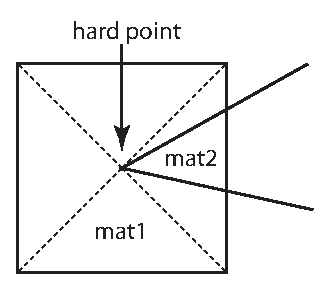
\includegraphics{quadtree/images/qdt_hard_point_demo_2.eps}
            }
        \caption{hard point is meshed as scaling center}
        \label{qdt_fig:qdt_hard_point_demo_sc}
        \end{subfigure}
        \caption[Example of a hard point]{Example of a hard point, elements around the point shared by three material must be properly divided into three.}
        \label{qdt_fig:qdt_hard_point_demo}
    \end{figure}
The difficulty in treating a hard point will be the position of itself in the background mesh.
The further it is away from the geometric center of the background mesh, the poorer the quality of mesh will be generated.
If the hard point in fig.~\ref{qdt_fig:qdt_hard_point_demo_sc} is located somewhere that is very close to the left boundary of the background mesh, the mesh for material one after cutting may be a quite elongated and twisted concave unit.
Besides, the requirement of the scaling center in the SBFEM can always be satisfied no matter where it is located in a convex polygon.
The opposite is true for a concave polygon, special treatment must be adopted to fullfil this requirement.
As a consequence, generally speaking, a convex mesh may always be preferred over a concave one and hard point can be the only source that will introduce concave polygons in most of the situation.
Although algorithm finding qualified scaling center in a concave polygon exists, the quality of the mesh may not be satisfactory even the scaling center is located on the vertex.


\paragraph{}
% make sure the hard point is close to the center of the background mesh
The first step to treat the hard point will be trying to locate the background mesh so that the hard point is close enough to its geometric center.
The ideal size of the background mesh shall ensure that only one hard point is in it and that no points from any other curves should be located in it.
As a consequence, the size of the containing square $box\_size$ is set to be one third of the distance to the nearest curves or half of the distance to the nearest hard point, whichever is smaller.
These parameter usually result in a valid and large enough background mesh that can treat the hard point easily. 
When building the background cell containing hard point in the algorithm, it will be implemented by have a considerably fine mesh within the range of the hard point and merge all cells in that range into one larger cell to be the background one.
Size of the ``considerably fine'' mesh $size\_field$ will be defined with the adjacent vertexes of the hard point as in eq.~\ref{qdt_eq:qdt_hard_point_size_field}
    \begin{equation}
        size\_field = \frac{box\_size}{
            2^{
                round(
                    \log(\frac{2 \pi}{ min(\alpha)})-1
                )
            }
        }
    \label{qdt_eq:qdt_hard_point_size_field}
    \end{equation}
where $\alpha$ is the minimal angle $min(\alpha_1, \alpha_2, \dots, \alpha_n)$ in fig.~\ref{qdt_fig:qdt_hard_point_setp_1}.
As is exponentially related to the minimal angle $\alpha$, the $size\_field$ may always be small enough to capture thin shell.
    \begin{figure}
        \centering
        \scalebox{0.5}{
            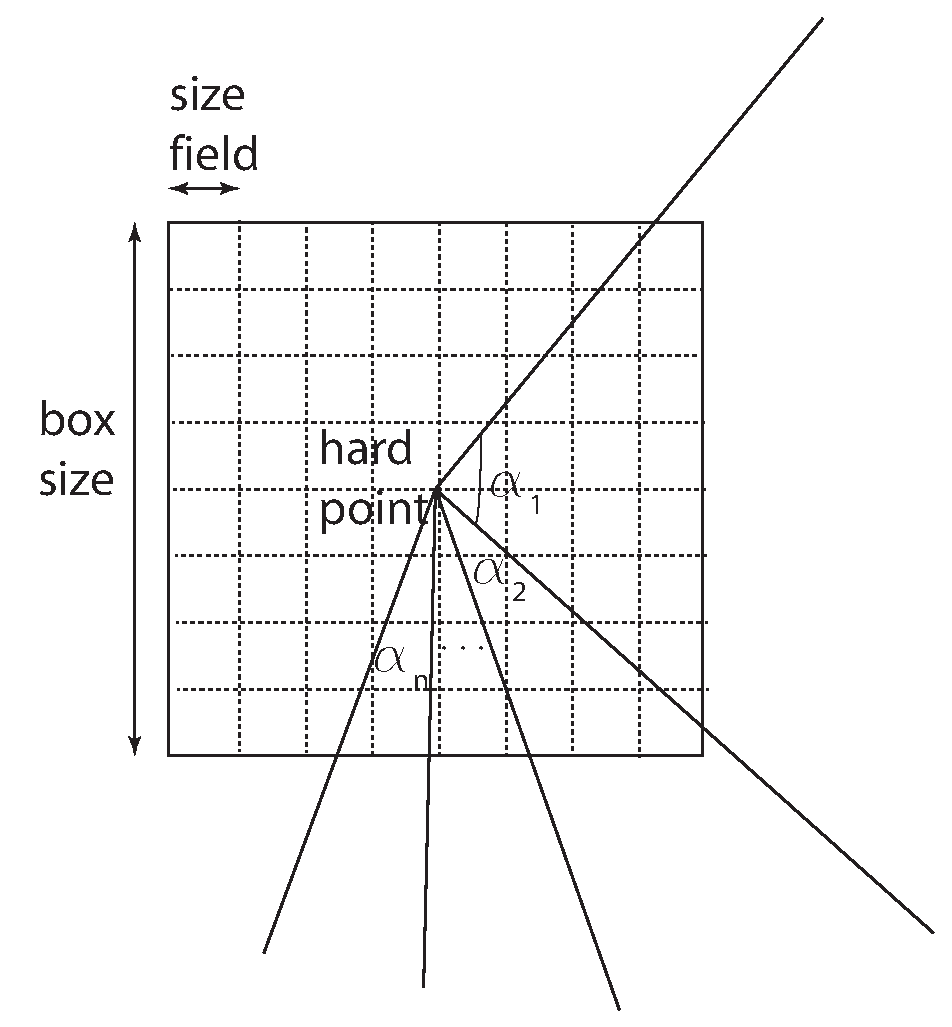
\includegraphics{quadtree/images/qdt_hard_point_step_1.eps}
        }
        \caption[Hard point treatment step 1]{Hard point treatment step1: find $box\_size$ and $size\_field$}
        \label{qdt_fig:qdt_hard_point_setp_1}
    \end{figure}

After the first step of the hard point treatment is done, the background cell shall have the following properties
    \begin{enumerate}
        \item Distance between hard point to geometric center of the background cell must be smaller than $\sqrt{2}size\_field$
        \item Element after cutting share the hard point as the node or it will be one element with scaling center located at the hard point
    \end{enumerate}
With these two properties, the cell can be cut by simply connecting the intersections with the hard point later.
\pagebreak


%=====================================================================================================================%
\subsection{Bucket sort algorithm}
\paragraph{}
When cutting the boundary, it is necessary to find the intersections between input geometry and the background mesh.
Finding geometric relationship between each cell and each curve may be necessary.
However, it could be computational expansive when quite a few curves are involved and a fine mesh is targeted.
As a result, an algorithm inspired by buck sort is introduced in order to reduce the computational cost of this process.
\paragraph{}
% introduce bucket sort algorithm
Bucket sort algorithm is a sorting algorithm that put an array of objects into different buckets and then sort the objects in each bucket.
Objects in each bucket then are sorted by other sorting algorithm or by applying buckets sort recursively.
Although the sort algorithm can not be adopted directly in finding the intersection, the idea ``divide and conquer'' can be utilized in order to help reduce the computational cost in finding the intersection.
\paragraph{}
% bucket sort in quadtree
First step of this method would be very similar to the first step in generating the background mesh.
The entire background square or the root of the quadtree will be divided evenly into $2^n \times 2^n$ smaller ones.
A larger $n$ will result in more buckets and will detect more irrelevant curves but take more time.
Trade off normally is not necessary and $n=8$ usually provide a good enough result so it can be fixed as $8$ unless special need is posed on.
Fig.~\ref{qdt_fig:qdt_bucket_sort} illustrates an example of the algorithm ($n$ is taken as $4$ in this example in order to have a clear figure, it should usually be taken as no less than $6$).
The end points of the curve are located in gird D2 and I5, as a consequence, the curve will be put in bucket ``D2-I5''.
In other words, cells that are not in this region shall not have any intersections with the curve.

\begin{figure}[!ht]
    \centering
    \scalebox{0.8}{
        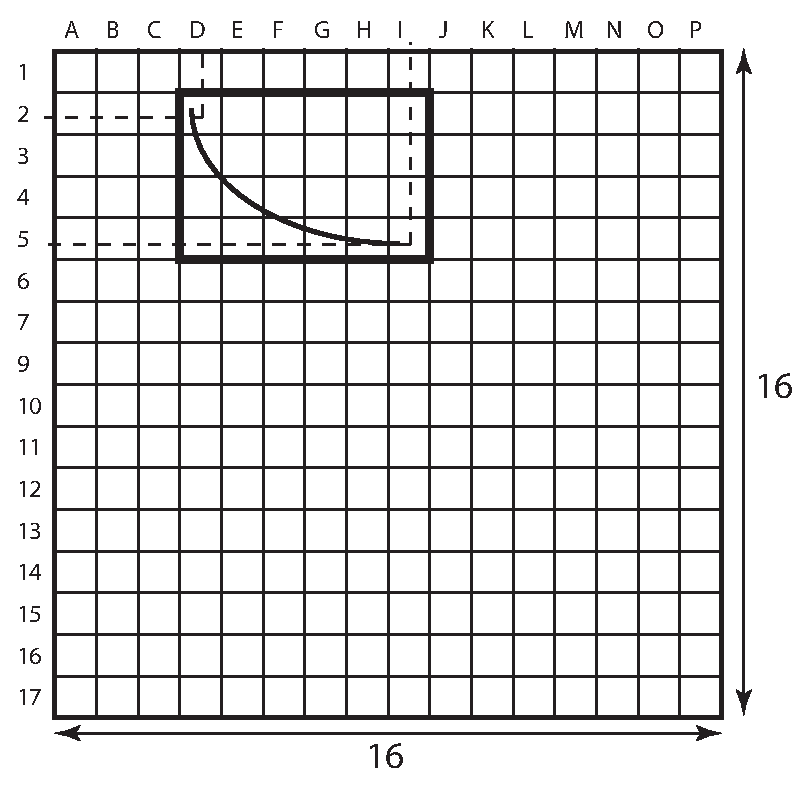
\includegraphics{quadtree/images/qdt_bucket_sort.eps}
    }
    \label{qdt_fig:qdt_bucket_sort}
    \caption[Bucket sort in quadtree]{Bucket sort in quadtree}
\end{figure}


\pagebreak
%=====================================================================================================================%
\subsection{Cutting with boundary}
\paragraph{}
% 3cases of the cutting
Generally, there are three situations where cutting is involved with one curve and they are sorted by the number of the intersections as shown in fig.~\ref{qdt_fig:qdt_cutting}.
Due to the fact that the background cell is refined properly and hence curves can be regarded as straight lines.
Case 3 in fig.~\ref{qdt_fig:qdt_cutting_3} is an exception as it shall not happen unless even the minimal allowable background cell may not able to catch the feature.
Unfortunately, result from case 3 may not be as expected and increase the resolution or decrease the minimal allowable cell size can help to prevent case 3 from happening.
\begin{figure}[!ht]
    \begin{subfigure}[b]{0.3\linewidth}
        \scalebox{1}{
            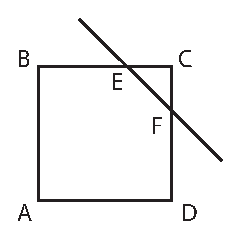
\includegraphics{quadtree/images/qdt_cutting_case_1.eps}
        }
        \caption{Case1: two intersections}
        \label{qdt_fig:qdt_cutting_2}
    \end{subfigure}
    \begin{subfigure}[b]{0.3\linewidth}
        \scalebox{1}{
            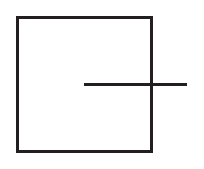
\includegraphics{quadtree/images/qdt_cutting_case_2.eps}
        }
        \label{qdt_fig:qdt_cutting_1}
        \caption{Case2: one intersectoin}
    \end{subfigure}
    \begin{subfigure}[b]{0.3\linewidth}
        \scalebox{1}{
            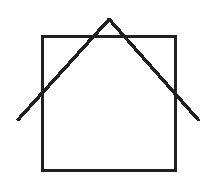
\includegraphics{quadtree/images/qdt_cutting_case_3.eps}
        }
        \caption{Case3: more than two intersections}
        \label{qdt_fig:qdt_cutting_3}
    \end{subfigure}
    \caption[Situations in cutting]{Situations in cutting: one, two and more than two intersections}
    \label{qdt_fig:qdt_cutting}
\end{figure}

\paragraph{}
% situation a (two intersections)
% sup an alg
In situation a (fig.~\ref{qdt_fig:qdt_cutting_2}) where two intersections are observed, cell can be split by connecting points $EF$.
To start with, any vertex among A, B, C or D can be selected as the start point.
After the point is selected, point A for example, another point from any of the line connected it will be chosen, point B for line AB for example.
This procedure will be repeated recursively until intersection point E or F is found and next point will be E or F whichever is not selected at the moment.
Recursion will be continued until the starting point is found again.
A closed region then will be formed by all selected points in sequence.
Another cell can also be easily be found by finding the implement set.
It should be noted that all cells split in situation must be convex.

\paragraph{}
% situation b (one intersection)
% sup an alg
In case 2 where only one intersection will be detected, multiple curves with intersection should be observed as in fig.~\ref{qdt_fig:qdt_cutting_hard_point} and hard point must be involved (point H in fig.~\ref{qdt_fig:qdt_cutting_hard_point}).
    \begin{figure}
        \centering
        \scalebox{1}{
            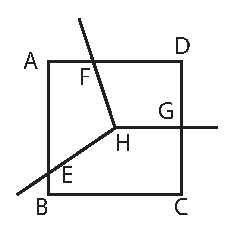
\includegraphics{quadtree/images/qdt_cutting_hard_point.eps}
        }
        \caption[Hard point treatment in cutting]{Hard point treatment in cutting}
        \label{qdt_fig:qdt_cutting_hard_point}
    \end{figure}
Handling case 2 would be similar but slightly tricky compared to that in case 1.
At the beginning, hard point is selected (point H in the example).
After that, any intersection point is selected (F in this example).
Then, the other point of any line segment that has F will be selected (D in this example).
The former step will be performed recursively until another intersection point is found under which situation.
Once the hard point is detected again, a closed region is found.
Repeat the procedure can find all closed region cut by hard point and multiple curves.

\paragraph{}
% situation c (more than two intersection)
% no alg needed
In case 3 where more than two intersections are found, result split cells may not be as expected as this situation shall not happen normally.
If case 3 does happen, the first and the last intersection points will be selected and all other intersection points will be ignored.
After that, method in case one can be applied directly.


\pagebreak
%=====================================================================================================================%
\subsection{Points moving}
\paragraph{}
% poor mesh quality
Although all types of cells with intersections are able to be treated by the algorithm described above, quality of the mesh sometimes may out of control as example shown in fig.~\ref{qdt_fig:qdt_cutting_poor_mesh_quality}.
    \begin{figure}[!ht]
        \centering
        \scalebox{1}{
            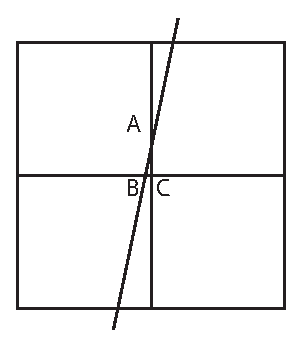
\includegraphics{quadtree/images/qdt_cutting_point_moving.eps}
        }
        \caption[Poor quality of mesh]{Poor quality of mesh: triangle element ABC is too small compared to its neiboughre}
        \label{qdt_fig:qdt_cutting_poor_mesh_quality}
    \end{figure}
\paragraph{}
% point moving
In order to improve the mesh quality, points moving is adopted.
Generally there are two ways of moving the points, one is move closing points to the line (move point C to line AB in fig.~\ref{qdt_fig:qdt_cutting_poor_mesh_quality}) and another is move points on the line to the closing point, e.g. point B will move to C in fig.~\ref{qdt_fig:qdt_cutting_poor_mesh_quality}.
Both method has its own advantages and disadvantage and will be discussed later.
\paragraph{}
% mark node as intersection
The recommended method is to mark the node that is close enough to the curve as intersection and project it back onto the curve at the end.
One significant advantage is that only convex cells may appear during cutting but special treatment need to be added in generating the background mesh.
The algorithm for cutting a convex cell into two will always yield valid result in existing algorithm.
For example, point C in fig.~\ref{qdt_fig:qdt_cutting_poor_mesh_quality} will be marked as intersection and point A and B will be ignored.
Point C will be projected back to the curve when the cutting is finished.
The threshold usually is taken as a proportion to the length of the background cell size.
When finding the intersection, another detection will be posed after.
If the distance of the intersection to a node is smaller than $\epsilon a$ where $\epsilon$ is tolerance and $a$ is the size of the background cell, the intersection will be ignored and the nearest node will be marked as intersection instead.
\begin{figure}
    \centering
    \scalebox{1}{
        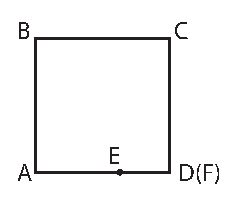
\includegraphics{quadtree/images/qdt_cutting_point_moving_1.eps}
    }
    \caption[Treatment of cell cutting when point is moved]{Treatment of cell cutting when point is moved}
    \label{qdt_fig:qdt_cutting_point_moving_1}
\end{figure}

\paragraph{}
Fig.~\ref{qdt_fig:qdt_cutting_point_moving_1} illustrates an example when points are moved toward one of the nodes.
If both intersections are moved then cutting may not be needed.
When one is moved and another is retained, algorithm described in previous section can be adopted directly as the topology remain the same.
The disadvantage is that it need to be taken into consideration when generating the background mesh as situation in fig.~\ref{qdt_fig:qdt_cutting_point_moving_problem}.
Points A, B and C will be marked as intersections and it becomes situation 3 in fig.~\ref{qdt_fig:qdt_cutting_3}.
However, background cell like it shall be refined otherwise unexpected behavior resulted from cutting algorithm may appear and such unexpected behavior shall be only allowed to happen when minimal allowable cell size in setting is too large to capture the local feature.
As a consequence, when refining background mesh in section.~\ref{qdt_sc:qdt_background_mesh}, not only the number of intersections between curves with the origin cell need to be counted, but also that from the enlarged box need to be counted as well as shown in fig.~\ref{qdt_fig:qdt_cutting_enlarged_box_point_moving_problem}.
Either more than two intersections are found in origin cell or the enlarged one in fig.~\ref{qdt_fig:qdt_cutting_enlarged_box} will result in the refinement of the cell.
\begin{figure}
    \begin{subfigure}[b]{0.5\linewidth}
        \centering
        \scalebox{1}{
            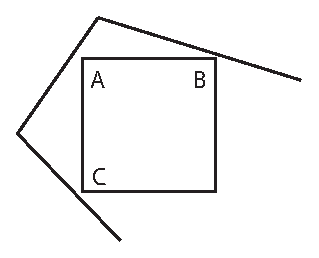
\includegraphics{quadtree/images/qdt_cutting_point_moving_1_dis.eps}
        }
        \caption{Problem in marking intersection}
        \label{qdt_fig:qdt_cutting_point_moving_problem}
    \end{subfigure}
    \begin{subfigure}[b]{0.5\linewidth}
        \centering
        \scalebox{1}{
            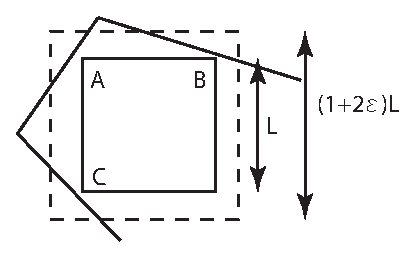
\includegraphics{quadtree/images/qdt_cutting_point_moving_1_enlarge.eps}
        }
        \caption{Enlarged box (dashed line)}
        \label{qdt_fig:qdt_cutting_enlarged_box}
    \end{subfigure}
    \caption[Problem in marking intersection]{Adopting enlarged box to ensure the background mesh is refined properly}
    \label{qdt_fig:qdt_cutting_enlarged_box_point_moving_problem}
\end{figure}

\paragraph{}
% move points before cutting
Another method is projecting the nodes in background mesh on to the curves before the cutting.
Special treatment in generating the background mesh is no longer necessary but cutting concave cells may be inevitable.
Fig.~\ref{qdt_fig:qdt_cutting_point_moving_2_concave} illustrates an example of a concave cell resulted from point moving.
An intersecting curve that is not a straight line even with a very small curvature, possibility exists that distance $a$ from the hanging node $A$ to the curve is slightly smaller than the tolerance while $b$ and $c$ are slightly larger than tolerance.
    \begin{figure}[!ht]
        \begin{subfigure}[b]{0.5\linewidth}
            \centering
            \scalebox{1.2}{
                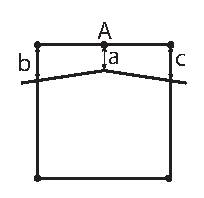
\includegraphics{quadtree/images/qdt_cutting_point_moving_2_concave_before.eps}
            }
            \caption{Before moving}
            \label{qdt_fig:qdt_cutting_point_moving_2_concave_before}
        \end{subfigure}
        \begin{subfigure}[b]{0.5\linewidth}
            \centering
            \scalebox{1.2}{
                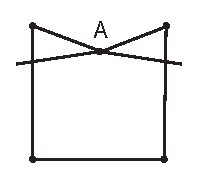
\includegraphics{quadtree/images/qdt_cutting_point_moving_2_concave_after.eps}
            }
            \caption{After moving}
            \label{qdt_fig:qdt_cutting_point_moving_2_concave_after}
        \end{subfigure}
        \caption[Concave cell resulted from points moving]{Concave cell resulted from point moving}
        \label{qdt_fig:qdt_cutting_point_moving_2_concave}
    \end{figure}

\paragraph{}
As a result, points $A$ will be moved on the curves but the other two nodes will not and hence cutting a concave cell need to be treated.
This method is not recommended because special treatment on cutting concave cells need to be implemented and it could be much more complicated than that in previous method.
First of all, more than two intersections will be observed in fig.~\ref{qdt_fig:qdt_cutting_point_moving_2_concave_after} and it may be mixed with case 3 in fig.~\ref{qdt_fig:qdt_cutting_3}.
Moreover, the concave cell will be cut into three instead of two which create extra difference.

\pagebreak
%=====================================================================================================================%
\subsection{Scaling center for concave elements}



\pagebreak
%=====================================================================================================================%
\subsection{Color the region}



\pagebreak